\documentclass[11pt,a4paper]{article}
\usepackage[T1]{fontenc}
\usepackage[margin=23mm,top=20mm,bottom=21mm,footskip=11mm]{geometry}
\usepackage{amsmath,amssymb,mathtools}
\usepackage{newpxtext,newpxmath,microtype}
\usepackage{xcolor,tikz,fancyhdr}
\usetikzlibrary{arrows.meta}
\definecolor{ink}{HTML}{182D38}
\definecolor{teal}{HTML}{006E70}
\definecolor{rust}{HTML}{AD482D}
\definecolor{muted}{HTML}{4C626B}
\definecolor{pale}{HTML}{EAF4F2}
\definecolor{rulecolor}{HTML}{BBD0D1}
\newcommand{\vct}[1]{\mathbf{#1}}
\newcommand{\T}{^{\mathsf T}}
\newcommand{\h}{\vct h}
\newcommand{\dirvec}{\vct v}
\newcommand{\q}{\vct q}
\newcommand{\stephead}[2]{\par\addvspace{9pt}\noindent{\large\sffamily\bfseries\color{teal}#1\quad #2}\par\nobreak\vspace{3pt}}
\newcommand{\ptitle}[1]{{\fontsize{24}{27}\selectfont\bfseries #1\par}\vspace{4pt}}
\newcommand{\kicker}[1]{{\footnotesize\sffamily\bfseries\color{teal}\MakeUppercase{#1}\par}\vspace{7pt}}
\pagestyle{fancy}\fancyhf{}
\fancyfoot[L]{\footnotesize\sffamily\color{muted}Residual-stream interventions}
\fancyfoot[R]{\footnotesize\sffamily\color{muted}\thepage\,/\,2}
\renewcommand{\headrulewidth}{0pt}
\renewcommand{\footrulewidth}{0.35pt}
\setlength{\parindent}{0pt}
\setlength{\parskip}{3pt}
\setlength{\abovedisplayskip}{6pt}
\setlength{\belowdisplayskip}{6pt}
\usepackage[pdfauthor={},pdftitle={Simultaneous ablation of non-orthogonal feature directions},hidelinks]{hyperref}
\begin{document}
\color{ink}
\kicker{Linear algebra for interpretability}
\ptitle{Simultaneous ablation of\\non-orthogonal feature directions}
\stephead{1}{The activation and the directions}
At one token and layer of an LLM, let $\h\in\mathbb R^d$ be the residual-stream activation. Let $\dirvec_1$ and $\dirvec_2$ be unit column vectors in that space. Bold lowercase letters denote vectors, uppercase letters denote matrices, and $^{\mathsf T}$ denotes transpose. As a running example, imagine one direction tracks quotation marks and the other tracks dialogue. Passages of quoted speech might activate both.
\stephead{2}{What should remain?}
Suppose we want to test how the model's next-token prediction changes when both direction scores are zero. We seek an edited activation $\h'$ with
\[
\dirvec_1\T\h'=\dirvec_2\T\h'=0,
\qquad \h-\h'\in\operatorname{span}(\dirvec_1,\dirvec_2).
\]
The second condition preserves every component perpendicular to the feature span. Together the conditions pick the closest qualifying activation to $\h$.
\stephead{3}{Why two subtractions can leak}
For a unit direction $\dirvec$, the scalar $\dirvec\T\h$ is its signed score. A first guess is to measure both scores on the original activation and subtract both projections. This gives
\[
\h_{\rm guess}=\h-(\dirvec_1\T\h)\dirvec_1-(\dirvec_2\T\h)\dirvec_2.
\]
The first subtraction clears the first score. After the second, that score is
$\dirvec_1\T\h_{\rm guess}=-(\dirvec_2\T\h)(\dirvec_1\T\dirvec_2)$. If the directions are orthogonal, the second move has no component along the first. Otherwise, the overlap $\dirvec_1\T\dirvec_2$ explains why the first score can return.

\textbf{What if we remeasure after the first edit?} In a sequential pass, let $\vct r=\h-(\dirvec_1\T\h)\dirvec_1$, then $\h_{\rm seq}=\vct r-(\dirvec_2\T\vct r)\dirvec_2$. This clears the second score, but the last move can still change the first one.
\par\vspace{6pt}
\noindent\begin{minipage}[c]{.50\linewidth}
\centering
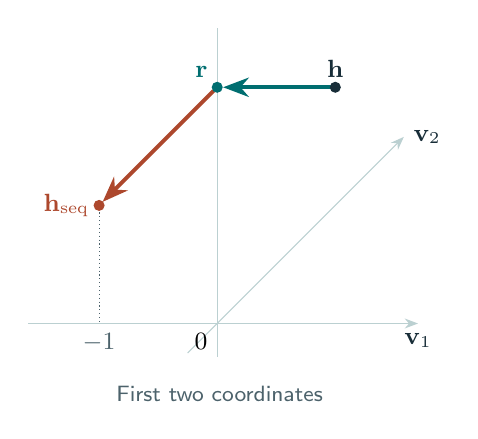
\begin{tikzpicture}[x=1.50cm,y=1.50cm,>=Stealth,font=\small]
\draw[rulecolor,->] (-1.6,0)--(1.70,0) node[below,ink] {$\dirvec_1$};
\draw[rulecolor] (0,-.28)--(0,2.5);
\draw[rulecolor,->] (-.25,-.25)--(1.58,1.58) node[right,ink] {$\dirvec_2$};
\draw[teal,line width=1.4pt,->] (.96,2)--(.05,2);
\draw[rust,line width=1.4pt,->] (-.03,1.97)--(-.97,1.03);
\fill[ink] (1,2) circle(2pt) node[above] {$\h$};
\fill[teal] (0,2) circle(2pt) node[above left] {$\vct r$};
\fill[rust] (-1,1) circle(2pt) node[left] {$\h_{\rm seq}$};
\draw[densely dotted,muted] (-1,.94)--(-1,0) node[below] {$-1$};
\node[below left] at (0,0) {$0$};
\node[below,font=\footnotesize\sffamily,text=muted] at (.02,-.45) {First two coordinates};
\end{tikzpicture}
\end{minipage}\hfill\begin{minipage}[c]{.48\linewidth}
\textbf{A diagonal move has a horizontal part.}
Take $\dirvec_1=(1,0,0)\T$, $\dirvec_2=(1,1,0)\T/\sqrt{2}$ and $\h=(1,2,3)\T$. The first edit gives $\vct r=(0,2,3)\T$. Its projection onto $\dirvec_2$ is $(1,1,0)\T$. Subtracting it takes one step left and one down, leaving $\h_{\rm seq}=(-1,1,3)\T$. The horizontal score went from zero to $-1$.
\end{minipage}
\newpage
\kicker{Simultaneous feature ablation}
\ptitle{Remove the shared span once}
\stephead{4}{Build an orthonormal basis with Gram--Schmidt}
Keep the first direction. From the second, subtract the part parallel to the first, then normalize the remainder. For independent directions this gives
\[
\q_1=\dirvec_1,\qquad \vct u_2=\dirvec_2-(\q_1\T\dirvec_2)\q_1,\qquad
\q_2=\frac{\vct u_2}{\lVert\vct u_2\rVert}.
\]
The new axes $\q_1,\q_2$ are perpendicular \emph{to each other} and span the same plane as $\dirvec_1,\dirvec_2$. Removing a component along $\q_2$ now preserves the zero score along $\q_1$. If $\vct u_2=\vct 0$, the first direction already spans both.
\stephead{5}{Orthonormal directions give the coefficients directly}
Stack $k$ unit directions as columns of $V=[\dirvec_1\ \cdots\ \dirvec_k]$. When they are mutually orthogonal, the coefficients to subtract are their signed scores. In matrix form,
\[
\vct a=V\T\h=(\dirvec_1\T\h,\ldots,\dirvec_k\T\h)\T,
\qquad \h'=\h-V\vct a.
\]
This also works with the orthonormal columns $Q$ from Gram--Schmidt, giving $\h'=\h-Q(Q\T\h)$.
\stephead{6}{For overlapping directions, solve for the coefficients together}
Assume the $k$ columns of $V$ are linearly independent. Write $\h'=\h-V\vct a$ so the edit lies in their span. Choose $\vct a$ to make every final score zero.
\begin{align*}
V\T\h' &= \vct 0 &&\text{require all $k$ dot products to vanish}\\
V\T(\h-V\vct a) &= \vct 0 &&\text{substitute the edited activation}\\
V\T\h-(V\T V)\vct a &= \vct 0 &&\text{distribute the transpose factor}\\
(V\T V)\vct a &= V\T\h &&\text{collect the unknown coefficients}\\
\vct a &= (V\T V)^{-1}V\T\h &&\text{solve the linear system.}
\end{align*}
The Gram matrix $G=V\T V$ has entries $G_{ij}=\dirvec_i\T\dirvec_j$. Its off-diagonal entries tell us how subtracting along one direction changes another's score.
\par\smallskip
{\setlength{\fboxsep}{8pt}\noindent\colorbox{pale}{\parbox{\dimexpr\linewidth-2\fboxsep\relax}{\centering
$\displaystyle \h'=\h-V(V\T V)^{-1}V\T\h
       =\bigl(I_d-V(V\T V)^{-1}V\T\bigr)\h.$}}}
\par\smallskip
Here $I_d$ is the $d$-dimensional identity. The matrix $P=V(V\T V)^{-1}V\T$ projects onto the feature span, so $I_d-P$ keeps its perpendicular complement. For dependent columns, use $P=QQ\T$ with an orthonormal basis $Q$ of that span.
\stephead{7}{Check the orthonormal case and the example}
If $V\T V=I_k$, the coefficients reduce to $V\T\h$ and $\h'=(I_d-VV\T)\h$. In the example, Gram--Schmidt gives the horizontal and vertical axes, so the simultaneous edit sends $(1,2,3)\T$ to $(0,0,3)\T$. The same edit in the original directions uses $\vct a=(-1,2\sqrt{2})\T$, since $-\dirvec_1+2\sqrt{2}\,\dirvec_2=(1,2,0)\T$. Both original scores vanish and the third coordinate survives.
\end{document}
